% Created by tikzDevice version 0.11 on 2018-04-11 18:36:10
% !TEX encoding = UTF-8 Unicode
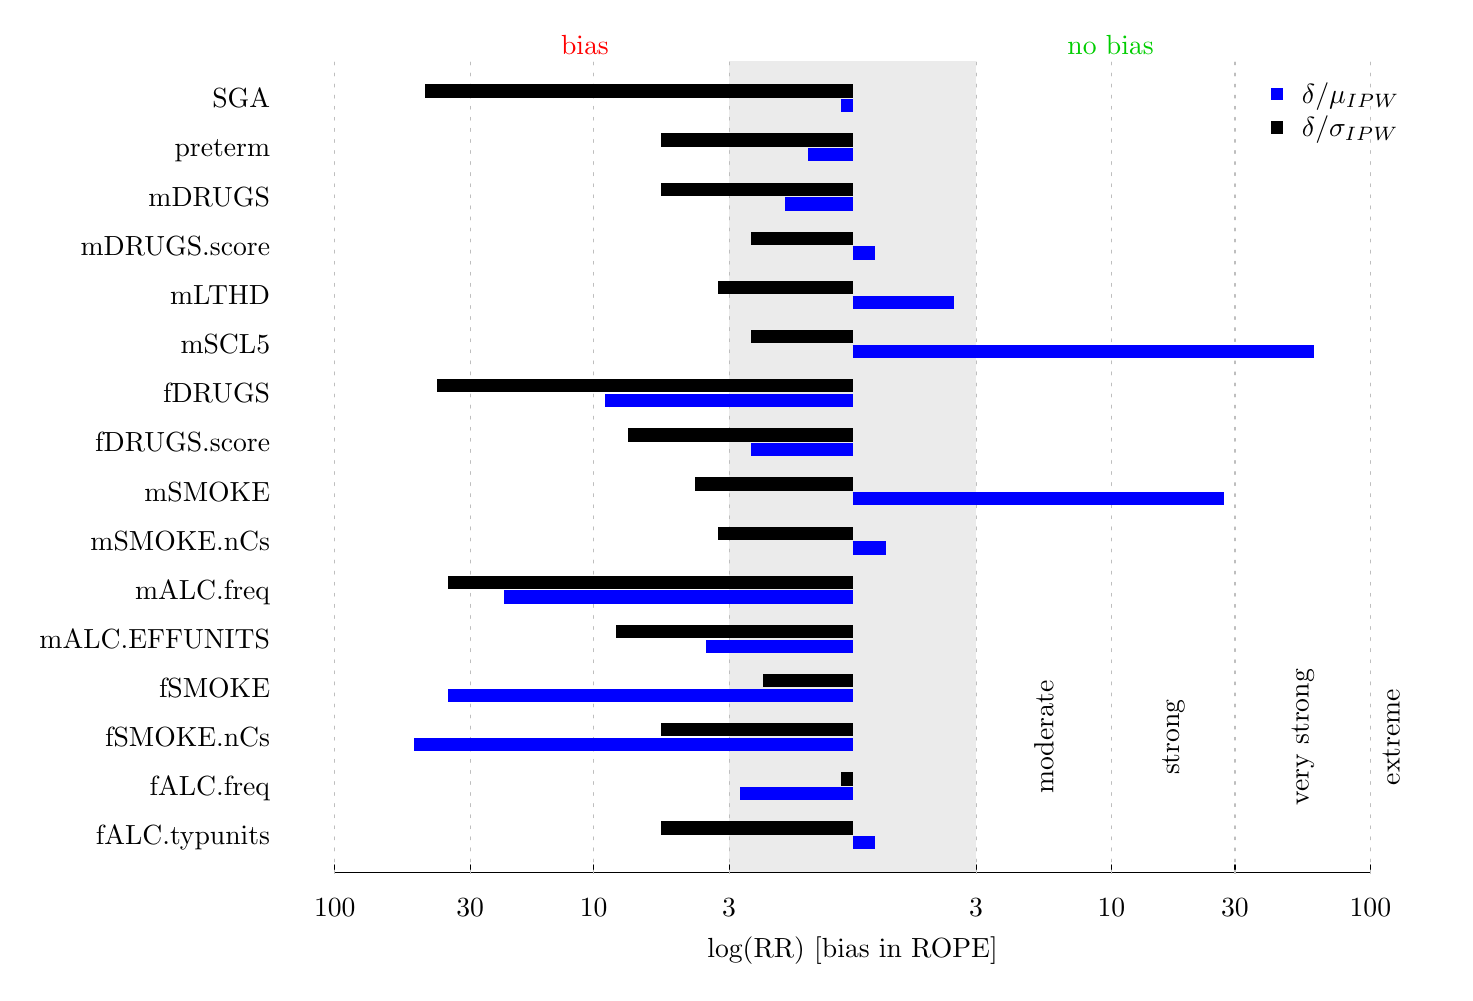
\begin{tikzpicture}[x=1pt,y=1pt]
\definecolor{fillColor}{RGB}{255,255,255}
\path[use as bounding box,fill=fillColor,fill opacity=0.00] (0,0) rectangle (512.15,341.43);
\begin{scope}
\path[clip] (  0.00,  0.00) rectangle (512.15,341.43);
\definecolor{drawColor}{RGB}{0,0,0}

\node[text=drawColor,anchor=base,inner sep=0pt, outer sep=0pt, scale=  1.00] at (298.07,  5.40) {log(RR) [bias in ROPE]};
\end{scope}
\begin{scope}
\path[clip] ( 96.00, 36.00) rectangle (500.15,329.43);
\definecolor{fillColor}{RGB}{190,190,190}

\path[fill=fillColor,fill opacity=0.30] (253.44, 36.00) rectangle (342.71,329.43);
\end{scope}
\begin{scope}
\path[clip] (  0.00,  0.00) rectangle (512.15,341.43);
\definecolor{drawColor}{RGB}{0,0,0}

\path[draw=drawColor,line width= 0.4pt,line join=round,line cap=round] (110.97, 36.00) -- (485.18, 36.00);

\path[draw=drawColor,line width= 0.4pt,line join=round,line cap=round] (110.97, 36.00) -- (110.97, 38.93);

\path[draw=drawColor,line width= 0.4pt,line join=round,line cap=round] (159.89, 36.00) -- (159.89, 38.93);

\path[draw=drawColor,line width= 0.4pt,line join=round,line cap=round] (204.52, 36.00) -- (204.52, 38.93);

\path[draw=drawColor,line width= 0.4pt,line join=round,line cap=round] (253.44, 36.00) -- (253.44, 38.93);

\path[draw=drawColor,line width= 0.4pt,line join=round,line cap=round] (342.71, 36.00) -- (342.71, 38.93);

\path[draw=drawColor,line width= 0.4pt,line join=round,line cap=round] (391.63, 36.00) -- (391.63, 38.93);

\path[draw=drawColor,line width= 0.4pt,line join=round,line cap=round] (436.26, 36.00) -- (436.26, 38.93);

\path[draw=drawColor,line width= 0.4pt,line join=round,line cap=round] (485.18, 36.00) -- (485.18, 38.93);

\node[text=drawColor,anchor=base,inner sep=0pt, outer sep=0pt, scale=  1.00] at (110.97, 20.40) {100};

\node[text=drawColor,anchor=base,inner sep=0pt, outer sep=0pt, scale=  1.00] at (159.89, 20.40) {30};

\node[text=drawColor,anchor=base,inner sep=0pt, outer sep=0pt, scale=  1.00] at (204.52, 20.40) {10};

\node[text=drawColor,anchor=base,inner sep=0pt, outer sep=0pt, scale=  1.00] at (253.44, 20.40) {3};

\node[text=drawColor,anchor=base,inner sep=0pt, outer sep=0pt, scale=  1.00] at (342.71, 20.40) {3};

\node[text=drawColor,anchor=base,inner sep=0pt, outer sep=0pt, scale=  1.00] at (391.63, 20.40) {10};

\node[text=drawColor,anchor=base,inner sep=0pt, outer sep=0pt, scale=  1.00] at (436.26, 20.40) {30};

\node[text=drawColor,anchor=base,inner sep=0pt, outer sep=0pt, scale=  1.00] at (485.18, 20.40) {100};
\end{scope}
\begin{scope}
\path[clip] ( 96.00, 36.00) rectangle (500.15,329.43);
\definecolor{drawColor}{RGB}{190,190,190}

\path[draw=drawColor,line width= 0.4pt,dash pattern=on 1pt off 3pt ,line join=round,line cap=round] (110.97, 36.00) -- (110.97,329.43);

\path[draw=drawColor,line width= 0.4pt,dash pattern=on 1pt off 3pt ,line join=round,line cap=round] (159.89, 36.00) -- (159.89,329.43);

\path[draw=drawColor,line width= 0.4pt,dash pattern=on 1pt off 3pt ,line join=round,line cap=round] (204.52, 36.00) -- (204.52,329.43);

\path[draw=drawColor,line width= 0.4pt,dash pattern=on 1pt off 3pt ,line join=round,line cap=round] (253.44, 36.00) -- (253.44,329.43);

\path[draw=drawColor,line width= 0.4pt,dash pattern=on 1pt off 3pt ,line join=round,line cap=round] (342.71, 36.00) -- (342.71,329.43);

\path[draw=drawColor,line width= 0.4pt,dash pattern=on 1pt off 3pt ,line join=round,line cap=round] (391.63, 36.00) -- (391.63,329.43);

\path[draw=drawColor,line width= 0.4pt,dash pattern=on 1pt off 3pt ,line join=round,line cap=round] (436.26, 36.00) -- (436.26,329.43);

\path[draw=drawColor,line width= 0.4pt,dash pattern=on 1pt off 3pt ,line join=round,line cap=round] (485.18, 36.00) -- (485.18,329.43);
\end{scope}
\begin{scope}
\path[clip] (  0.00,  0.00) rectangle (512.15,341.43);
\definecolor{drawColor}{RGB}{255,0,0}

\node[text=drawColor,anchor=base,inner sep=0pt, outer sep=0pt, scale=  1.00] at (201.36,331.83) {bias};
\definecolor{drawColor}{RGB}{0,205,0}

\node[text=drawColor,anchor=base east,inner sep=0pt, outer sep=0pt, scale=  1.00] at (406.90,331.83) {no bias};
\definecolor{drawColor}{RGB}{0,0,0}

\node[text=drawColor,anchor=base east,inner sep=0pt, outer sep=0pt, scale=  1.00] at ( 87.60, 46.09) {fALC.typunits};

\node[text=drawColor,anchor=base east,inner sep=0pt, outer sep=0pt, scale=  1.00] at ( 87.60, 63.85) {fALC.freq};

\node[text=drawColor,anchor=base east,inner sep=0pt, outer sep=0pt, scale=  1.00] at ( 87.60, 81.60) {fSMOKE.nCs};

\node[text=drawColor,anchor=base east,inner sep=0pt, outer sep=0pt, scale=  1.00] at ( 87.60, 99.36) {fSMOKE};

\node[text=drawColor,anchor=base east,inner sep=0pt, outer sep=0pt, scale=  1.00] at ( 87.60,117.12) {mALC.EFFUNITS};

\node[text=drawColor,anchor=base east,inner sep=0pt, outer sep=0pt, scale=  1.00] at ( 87.60,134.88) {mALC.freq};

\node[text=drawColor,anchor=base east,inner sep=0pt, outer sep=0pt, scale=  1.00] at ( 87.60,152.64) {mSMOKE.nCs};

\node[text=drawColor,anchor=base east,inner sep=0pt, outer sep=0pt, scale=  1.00] at ( 87.60,170.39) {mSMOKE};

\node[text=drawColor,anchor=base east,inner sep=0pt, outer sep=0pt, scale=  1.00] at ( 87.60,188.15) {fDRUGS.score};

\node[text=drawColor,anchor=base east,inner sep=0pt, outer sep=0pt, scale=  1.00] at ( 87.60,205.91) {fDRUGS};

\node[text=drawColor,anchor=base east,inner sep=0pt, outer sep=0pt, scale=  1.00] at ( 87.60,223.67) {mSCL5};

\node[text=drawColor,anchor=base east,inner sep=0pt, outer sep=0pt, scale=  1.00] at ( 87.60,241.43) {mLTHD};

\node[text=drawColor,anchor=base east,inner sep=0pt, outer sep=0pt, scale=  1.00] at ( 87.60,259.18) {mDRUGS.score};

\node[text=drawColor,anchor=base east,inner sep=0pt, outer sep=0pt, scale=  1.00] at ( 87.60,276.94) {mDRUGS};

\node[text=drawColor,anchor=base east,inner sep=0pt, outer sep=0pt, scale=  1.00] at ( 87.60,294.70) {preterm};

\node[text=drawColor,anchor=base east,inner sep=0pt, outer sep=0pt, scale=  1.00] at ( 87.60,312.46) {SGA};
\end{scope}
\begin{scope}
\path[clip] ( 96.00, 36.00) rectangle (500.15,329.43);
\definecolor{drawColor}{RGB}{0,0,255}

\path[draw=drawColor,line width= 4.8pt,line join=round] (298.07,313.24) -- (294.01,313.24);

\path[draw=drawColor,line width= 4.8pt,line join=round] (298.07,295.48) -- (281.82,295.48);

\path[draw=drawColor,line width= 4.8pt,line join=round] (298.07,277.72) -- (273.70,277.72);

\path[draw=drawColor,line width= 4.8pt,line join=round] (298.07,259.96) -- (306.20,259.96);

\path[draw=drawColor,line width= 4.8pt,line join=round] (298.07,242.21) -- (334.64,242.21);

\path[draw=drawColor,line width= 4.8pt,line join=round] (298.07,224.45) -- (464.66,224.45);

\path[draw=drawColor,line width= 4.8pt,line join=round] (298.07,206.69) -- (208.69,206.69);

\path[draw=drawColor,line width= 4.8pt,line join=round] (298.07,188.93) -- (261.51,188.93);

\path[draw=drawColor,line width= 4.8pt,line join=round] (298.07,171.17) -- (432.15,171.17);

\path[draw=drawColor,line width= 4.8pt,line join=round] (298.07,153.42) -- (310.26,153.42);

\path[draw=drawColor,line width= 4.8pt,line join=round] (298.07,135.66) -- (172.12,135.66);

\path[draw=drawColor,line width= 4.8pt,line join=round] (298.07,117.90) -- (245.26,117.90);

\path[draw=drawColor,line width= 4.8pt,line join=round] (298.07,100.14) -- (151.81,100.14);

\path[draw=drawColor,line width= 4.8pt,line join=round] (298.07, 82.38) -- (139.62, 82.38);

\path[draw=drawColor,line width= 4.8pt,line join=round] (298.07, 64.63) -- (257.45, 64.63);

\path[draw=drawColor,line width= 4.8pt,line join=round] (298.07, 46.87) -- (306.20, 46.87);
\definecolor{drawColor}{RGB}{0,0,0}

\path[draw=drawColor,line width= 4.8pt,line join=round] (298.07,318.57) -- (143.68,318.57);

\path[draw=drawColor,line width= 4.8pt,line join=round] (298.07,300.81) -- (229.00,300.81);

\path[draw=drawColor,line width= 4.8pt,line join=round] (298.07,283.05) -- (229.00,283.05);

\path[draw=drawColor,line width= 4.8pt,line join=round] (298.07,265.29) -- (261.51,265.29);

\path[draw=drawColor,line width= 4.8pt,line join=round] (298.07,247.53) -- (249.32,247.53);

\path[draw=drawColor,line width= 4.8pt,line join=round] (298.07,229.78) -- (261.51,229.78);

\path[draw=drawColor,line width= 4.8pt,line join=round] (298.07,212.02) -- (147.75,212.02);

\path[draw=drawColor,line width= 4.8pt,line join=round] (298.07,194.26) -- (216.82,194.26);

\path[draw=drawColor,line width= 4.8pt,line join=round] (298.07,176.50) -- (241.19,176.50);

\path[draw=drawColor,line width= 4.8pt,line join=round] (298.07,158.74) -- (249.32,158.74);

\path[draw=drawColor,line width= 4.8pt,line join=round] (298.07,140.99) -- (151.81,140.99);

\path[draw=drawColor,line width= 4.8pt,line join=round] (298.07,123.23) -- (212.75,123.23);

\path[draw=drawColor,line width= 4.8pt,line join=round] (298.07,105.47) -- (265.57,105.47);

\path[draw=drawColor,line width= 4.8pt,line join=round] (298.07, 87.71) -- (229.00, 87.71);

\path[draw=drawColor,line width= 4.8pt,line join=round] (298.07, 69.95) -- (294.01, 69.95);

\path[draw=drawColor,line width= 4.8pt,line join=round] (298.07, 52.20) -- (229.00, 52.20);
\end{scope}
\begin{scope}
\path[clip] (  0.00,  0.00) rectangle (512.15,341.43);
\definecolor{drawColor}{RGB}{0,0,0}

\node[text=drawColor,rotate= 90.00,anchor=base,inner sep=0pt, outer sep=0pt, scale=  1.00] at (370.61, 85.05) {moderate};

\node[text=drawColor,rotate= 90.00,anchor=base,inner sep=0pt, outer sep=0pt, scale=  1.00] at (416.05, 85.05) {strong};

\node[text=drawColor,rotate= 90.00,anchor=base,inner sep=0pt, outer sep=0pt, scale=  1.00] at (462.83, 85.05) {very strong};

\node[text=drawColor,rotate= 90.00,anchor=base,inner sep=0pt, outer sep=0pt, scale=  1.00] at (495.74, 85.05) {extreme};
\definecolor{drawColor}{RGB}{255,255,255}

\path[draw=drawColor,line width= 0.4pt,line join=round,line cap=round] (442.45,329.43) rectangle (500.15,293.43);
\definecolor{fillColor}{RGB}{0,0,255}

\path[fill=fillColor] (449.20,315.18) --
	(453.70,315.18) --
	(453.70,319.68) --
	(449.20,319.68) --
	cycle;
\definecolor{fillColor}{RGB}{0,0,0}

\path[fill=fillColor] (449.20,303.18) --
	(453.70,303.18) --
	(453.70,307.68) --
	(449.20,307.68) --
	cycle;
\definecolor{drawColor}{RGB}{0,0,0}

\node[text=drawColor,anchor=base west,inner sep=0pt, outer sep=0pt, scale=  1.00] at (460.45,313.99) {$\delta/\mu_{IPW}$};

\node[text=drawColor,anchor=base west,inner sep=0pt, outer sep=0pt, scale=  1.00] at (460.45,301.99) {$\delta/\sigma_{IPW}$};
\end{scope}
\end{tikzpicture}
